\def\labauthors{Карусевич А.А., Понур К.А.}
\def\labgroup{440}
\def\labnumber{1}
\def\labtheme{Колебания механических систем \\[0.2em] с распределенными параметрами}
\def\shortlabtheme{Колебания пластин и стержней}
\def\department{Кафедра акустики}
% Тип документа
\documentclass[a4paper,12pt]{extarticle}

% Шрифты, кодировки, символьные таблицы, переносы
% \usepackage{cmap}
% \usepackage[T2A]{fontenc}
\usepackage[utf8]{inputenc}
\usepackage[russian]{babel}
% Это пакет -- хитрый пакет, он нужен но не нужен
\usepackage[mode=buildnew]{standalone}

\usepackage
	{
		% Дополнения Американского математического общества (AMS)
		amssymb,
		amsfonts,
		amsmath,
		amsthm,
		% Пакет для физических текстов
		physics,
		% misccorr,
		% 
		% Графики и рисунки
		wrapfig,
		graphicx,
		subcaption,
		float,
		caption,
		csvsimple,
		color,
		booktabs,
		geometry,
		% 
		% Таблицы, списки
		makecell,
		multirow,
		indentfirst,
		%
		% Интегралы и прочие обозначения
		ulem,
		esint,
		esdiff,
		% 
		% Колонтитулы
		fancyhdr,
	} 
    
\usepackage{mathtools}
\mathtoolsset{showonlyrefs=true} 
\usepackage{pgfplots,pgfplotstable,booktabs,colortbl}
\usepackage{xcolor}
\usepackage{hyperref}
\usepackage{pythontex}
 % Цвета для гиперссылок
\definecolor{linkcolor}{HTML}{000000} % цвет ссылок
\definecolor{urlcolor}{HTML}{799B03} % цвет гиперссылок
 
\hypersetup{pdfstartview=FitH,linkcolor=linkcolor,urlcolor=urlcolor, colorlinks=true}
\hypersetup{pageanchor=false}
% Увеличенный межстрочный интервал, французские пробелы
\linespread{1.3} 
\frenchspacing 

\newcommand{\mean}[1]{\langle#1\rangle}

\begin{pycode}

def frexp10(decimal):
	parts = ('%e' % decimal).split('e')
	return float(parts[0]), int(parts[1])

\end{pycode}



% Функция для тех, кто использует pythontex. Представляет любое вещественное число в стандартном виде.
\newcommand{\frexp}[1]{
		\pyc{#10=frexp10(#1)} 
			\py{ round(#10[0],2)} 
				\cdot 10^{\py{#10[1]}} }

% const прямым шрифтом
\newcommand\ct[1]{\text{\rmfamily\upshape #1}}
\newcommand*{\const}{\ct{const}}
\usepackage{array}
\usepackage{pstool}

\geometry		
	{
		left			=	2cm,
		right 			=	2cm,
		top 			=	2.5cm,
		bottom 			=	2.5cm,
		bindingoffset	=	0cm
	}

%%%%%%%%%%%%%%%%%%%%%%%%%%%%%%%%%%%%%%%%%%%%%%%%%%%%%%%%%%%%%%%%%%%%%%%%%%%%%%%
	%применим колонтитул к стилю страницы
\pagestyle{fancy} 
	%очистим "шапку" страницы
% \fancyhead{} 
	%слева сверху на четных и справа на нечетных
\fancyhead[R]{}%\labauthors 
	%справа сверху на четных и слева на нечетных
% \fancyhead[L]{Отчёт по лабораторной работе №\labnumber}
\fancyhead[L]{\shortlabtheme} 
	%очистим "подвал" страницы
% \fancyfoot{} 
	% номер страницы в нижнем колинтуле в центре
\fancyfoot[C]{\thepage} 

%%%%%%%%%%%%%%%%%%%%%%%%%%%%%%%%%%%%%%%%%%%%%%%%%%%%%%%%%%%%%%%%%%%%%%%%%%%%%%%

\renewcommand{\contentsname}{Оглавление}
\usepackage{tocloft}
\usepackage{secdot}
\sectiondot{subsection}


\begin{document}
\begin{titlepage}

\begin{center}

{\small\textsc{Нижегородский государственный университет имени Н.\,И. Лобачевского}}
\vskip 1pt \hrule \vskip 3pt
{\small\textsc{Радиофизический факультет}}



\vfill
{\Large {\department}}

{\Large Отчет по лабораторной работе №\labnumber\vskip 12pt\bfseries \labtheme}
	
\end{center}

\vfill
	
\begin{flushright}
	{Выполнили студенты \labgroup\ группы\\ \labauthors}%\vskip 12pt Принял:\\ Менсов С.\,Н.}
\end{flushright}
	
\vfill
	
\begin{center}
	Нижний Новгород, \the\year
\end{center}

\end{titlepage}


\tableofcontents
\newpage


\addcontentsline{toc}{section}{Введение}
\section*{Введение}
\vspace{-0.5em}
В настоящей работе исследуются продольные колебания стержней и поперечные колебания пластин с помощью резонансного метода -- возбуждаются колебания на резонансных частотах. Под пластиной понимается упругое трехмерное тело, один размер которого много меньше двух других, а под стержнем -- тело, у которого один размер больше двух других. 

В эксперименте используются три стержня (из алюминия, стали и оргстекла, все длины 394 мм) и две металлические пластины (толщины 0.63 мм и 1.16 мм)
\vspace{-0.5em}


\paragraph{Установка с стержнями.} Стержни закрепляются в неподвижном штативе, при этом точка крепления посередине стержня,  а к свободным торцам стержня на малом расстоянии поднесены электромагнитные вибраторы -- приемный и излучающий. Меняя частоту генератора, подключенного к излучающему вибратору, и измеряя амплитуду на приемном можно получить резонансные характеристики системы.

\paragraph{Установка с пластинами.} Металлическая пластина закреплена в станке, в котором размещен электромагнитный возбудитель колебаний. Возбудитель можно перемещать вдоль диаметра пластинки и наблюдать при этом различные типы колебаний. На пластине рассыпается тонкий слой песка, который при резонансе собирается в узлах колебаний пластины. Полученные картины называются картинами Хладни и позволяют определить конкретную моду колебаний.

% \begin{figure}[H]
% 	\centering
% 	\includegraphics[width=\textwidth]{fig/view}
% 	\vspace{-1em}
% 	\caption{Лабораторная установка. 1 -- осциллограф ОСУ-10А, 2 -- генератор сигналов UNI-T UTG9010C, 3 -- измерительный модуль, подключенный в режиме усилителя входного сигнала, 4 -- мультиметр APPA-201N, 5,6 -- источники питания GPS-3030D (в принципиальной схеме -- $E_2$, $E_1$).}
% 	\label{fig:1}
% \end{figure}

\newpage

\section{Резонансные кривые продольных колебаний}
\subsection{Алюминиевый стержень}
\begin{figure}[H]
	\centering
	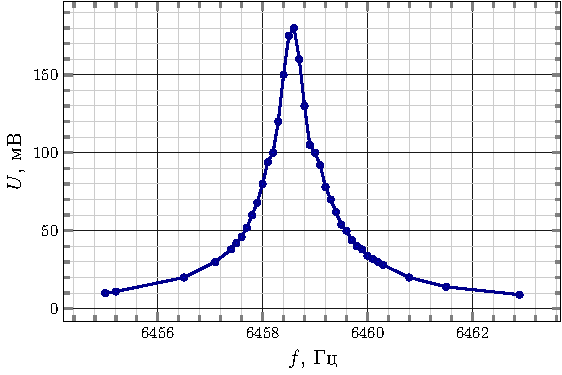
\includegraphics[scale=1.5]{fig/al_afc}
	\caption{Принципиальная схема}
	\label{fig:chem1}
\end{figure}

Из графика снятой АЧХ нашли параметры резонансной кривой: резонансную частоту
$f_0=6458.6\text{ Гц}$ и ширину на уровне 0.7 $\Delta f_{0.7} \approx 1\text{ Гц}$. 
Частота согласуется с теоретическим значением первой моды
\begin{equation}
	f_1 = \frac{1\cdot c}{2l} = \frac{5140 \text{ м}\cdot\text{с}^{-1}}{2\cdot 0.394\text{ м}}=6522 \text{ Гц}
\end{equation}
Добротность колебательной системы
\begin{equation}
	Q = \frac{f_0}{\Delta f_{0.7}} \approx 6450
\end{equation}
Исходя из табличного значения модуля Юнга для алюминия $E=0.07\cdot10^{12}$ Па, нашли вязкость стержня  \cite[стр. 10]{met}:
\begin{equation}
	\eta = \frac{\gamma E}{\omega_0}= \frac{ E}{Q 2\pi f_0} = \frac{\Delta f_{0.7} E}{2\pi f_0^2}= 270 \text{ кг}\cdot\text{м}^{-1}\cdot\text{с}^{-1}
\end{equation}

\subsection{Стержень из оргстекла}

\begin{figure}[H]
	\centering
	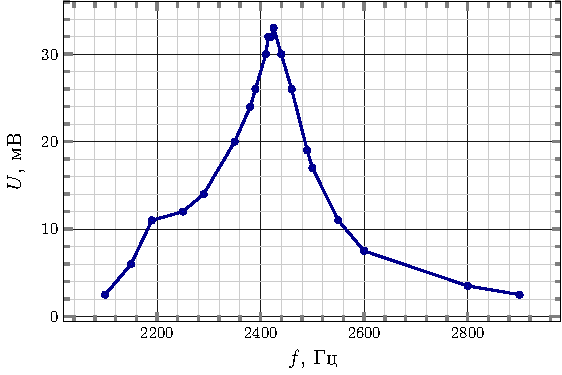
\includegraphics[scale=1.5]{fig/glass_afc}
	\caption{Резонансная кривая колебаний в стержне из оргстекла}
	\label{fig:chem1}
\end{figure}

Из графика снятой АЧХ нашли параметры резонансной кривой: резонансную частоту
$f_0=2420\text{ Гц}$ и ширину на уровне 0.7 $\Delta f_{0.7} = 96\text{ Гц}$. 
Частота согласуется с теоретическим значением первой моды
\begin{equation}
	f_1 = \frac{1\cdot c}{2l} = \frac{2040 \text{ м}\cdot\text{с}^{-1}}{2\cdot 0.394\text{ м}}=2588 \text{ Гц}
\end{equation}
Добротность колебательной системы
\begin{equation}
	Q = \frac{f_0}{\Delta f_{0.7}} \approx 25
\end{equation}
Исходя из табличного значения модуля Юнга для оргстекла $E=0.005\cdot10^{12}$ Па, нашли вязкость стержня  \cite[стр. 10]{met}:
\begin{equation}
	\eta = \frac{\gamma E}{\omega_0}= \frac{ E}{Q 2\pi f_0} = \frac{\Delta f_{0.7} E}{2\pi f_0^2} = 13150 \text{ кг}\cdot\text{м}^{-1}\cdot\text{с}^{-1}
\end{equation}


\subsection{Стальной стержень}

\begin{figure}[H]
	\centering
	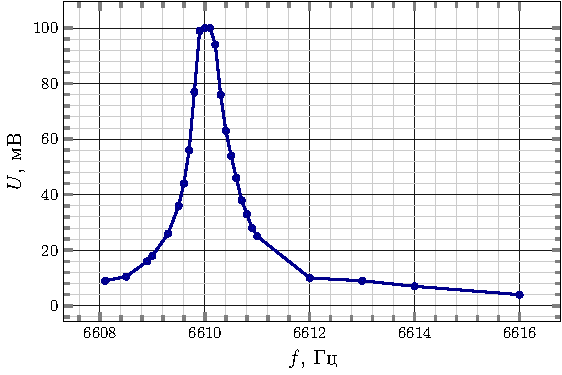
\includegraphics[scale=1.5]{fig/steel_afc.pdf}
	\vspace{-1em}
	\caption{Семейство переходных характеристик}
	\label{fig:2}
\end{figure}
Из графика снятой АЧХ нашли параметры резонансной кривой: резонансную частоту
$f_0=6610\text{ Гц}$ и ширину на уровне 0.7 $\Delta f_{0.7} = 0.48\text{ Гц}$. 
Частота хорошо согласуется с теоретическим значением первой моды
\begin{equation}
	f_1 = \frac{1\cdot c}{2l} = \frac{5210 \text{ м}\cdot\text{с}^{-1}}{2\cdot 0.394\text{ м}}=6611 \text{ Гц}
\end{equation}
Добротность колебательной системы
\begin{equation}
	Q = \frac{f_0}{\Delta f_{0.7}} \approx 13770
\end{equation}
Исходя из табличного значения модуля Юнга для стали $E=0.20\cdot10^{12}$ Па, нашли вязкость стержня  \cite[стр. 10]{met}:
\begin{equation}
	\eta = \frac{\gamma E}{\omega_0} = \frac{ E}{Q 2\pi f_0} = \frac{\Delta f_{0.7} E}{2\pi f_0^2} = 340 \text{ кг}\cdot\text{м}^{-1}\cdot\text{с}^{-1}
\end{equation}

\newpage
\subsection{Экспериментальное значение модуля Юнга}

В предыдущих пунктах значение модуля Юнга бралось apriori, а согласованность проверялась сравнением первых мод. Однако, можно рассчитать уточненное значение модуля Юнга, рассчитав в обратном порядке скорость звука в продольном стержне, исходя из экспериментальных данных:
\begin{equation}
	c=\frac{2l f_n}{n}=2lf_n=
	\left\{
	\begin{aligned}
		5089 \text{ м}\cdot\text{с}^{-1},&\quad \text{алюминий}\\
		1097 \text{ м}\cdot\text{с}^{-1},&\quad \text{оргстекло}\\
		5208 \text{ м}\cdot\text{с}^{-1},&\quad \text{сталь}
	\end{aligned}
	\right.
\end{equation}
Считая известными плотности, найдем модуль Юнга:
\begin{equation}
	E = \rho c^2=
	\left\{
	\begin{aligned}
		0.069\cdot 10^{12}\text{ Па},&\quad \text{алюминий}\\
		0.0014\cdot 10^{12}\text{ Па},&\quad \text{оргстекло}\\
		0.211\cdot 10^{12}\text{ Па},&\quad \text{сталь}
	\end{aligned}
	\right.
\end{equation}
Тогда уточнённое значение вязкости для стали и алюминия изменится в пределах погрешности измерений, а для оргстекла
\begin{equation}
	\eta_{new}\approx 3700 \text{ кг}\cdot\text{м}^{-1}\cdot\text{с}^{-1}
\end{equation}

Возникает вопрос о причине такого сильного расхождения. Это можно объяснить тем, что вычисляюся величины, опирающиеся на эксперимент, т.е. снятую резонансную кривую, которая характеризует не колебания в стержне, но и характеристики колебательной системы в целом, в том числе, приемника/передатчика.

\newpage

\section{Поперечные колебания круглых пластин}

В данном эксперименте изучались т.н. фигуры Хладни, образующиеся из скоплений частиц песка на колеблющейся пластине в узлах колебаний. Фигуры был получены на различных модах колебаний в пределах 0.5--1.5 кГц для двух пластин различной толщины при двух положениях излучателя.

\subsection{Пластина 0.63 мм}
\subsubsection{Излучатель в центре}
\begin{figure}[H]
	\centering
	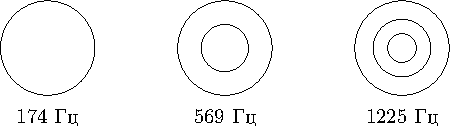
\includegraphics[scale=1.5]{fig/63_c.pdf}
\end{figure}
\subsubsection{Излучатель смещен}
\begin{figure}[H]
	\centering
	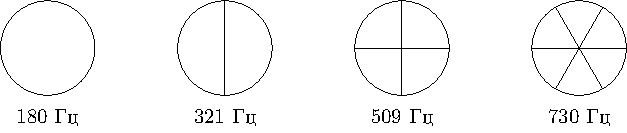
\includegraphics[scale=1.5]{fig/63_b.pdf}
\end{figure}
\subsection{Пластина 1.16 мм}
\subsubsection{Излучатель в центре}
\begin{figure}[H]
	\centering
	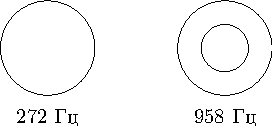
\includegraphics[scale=1.5]{fig/116_c.pdf}
\end{figure}
\subsubsection{Излучатель смещен}
\begin{figure}[H]
	\centering
	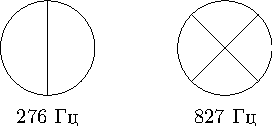
\includegraphics[scale=1.5]{fig/116_b.pdf}
\end{figure}

Можно отметить, что при смещении излучателя частота основного тона повышается. В каждом из экспериментов были сняты основной тон и один и более обертонов. Наиболее высокий обретон, который удалось получить -- $f_{31}$ для пластины 0.63 мм.

\subsection{Теоретические значения частот}
Собственные частоты изгибных колебаний пластины определяются формулой
\begin{equation}
	\omega_{mn} = \frac{\pi^2 H}{a^2}\beta_{mn}^2 \qty|\frac{E}{3\rho_s (1-\nu^2)}|^{\frac12}
\end{equation}

Где значения $\beta_{mn}$ порождаются решением уравнений относительно функций Бесселя и не связаны с характеристиками установки. $\beta_{mn}$ можно считать известными.

Так как некоторые константы были не известны, можно поступить следующим образом: брать основной тон из эксперимента и пытаться рассчитать по формуле обертона. Например, для основного тона $f_{01}=165$ Гц рассчитаем обертона $f_{02,03}$:
\begin{equation}
	f_{02} = 3.309 f_{01} = 545 \text{ Гц},\qquad 
	f_{03} = 2.234 f_{02} = 1217 \text{ Гц} 
\end{equation}
В эксперименте же наблюдались частоты 567 и 1226 Гц. Завышение теоретических значений можно объяснить наличием диссипации: так, по аналогии, учет диссипации для колебаний в LC-контуре приводит к уменьшению резонансной частоты.
\newpage
\addcontentsline{toc}{section}{Заключение}
\section*{Заключение}
В настоящей работе были изучены линейные теории двумерных колебательных систем с распределенными параметрами (пластин и стержней); проведен ряд экспериментов с пластинами и стержнями. 

Для стержней были получены резонансные кривые, рассчитаны добротность, модуль Юнга и коэффициент вязкости для каждого стержня. Следует отметить различие в ширинах резонансных кривых (и, как следствие, добротностях) для стали и оргстекла. Для оргстекла ширина резонансной кривой составляет несколько сотен Герц (и добротность $\sim10$), а для стали ширина кривой несколько Герц (а добротность $\sim 10^4$). Такая большая разница связана с различиями в структурах оргстекла и стали. Оргстекло -- аморфный материал с высокой (по сравнению со сталью) вязкостью, поэтому колебания в нем распространяются хуже, чем в стали. 

В экспериментах с пластинами были получены фигуры Хладни, определены моды колебаний для двух положений возбудителя: по центру пластины и сдвинутым относительно центра.

% \newpage
\begin{thebibliography}{}
  \bibitem{mss} Гурбатов С.Н. Лекции по механике сплошных сред на радиофизическом факультете 2018/2019. -- 106 с.
  
  \bibitem{met} Горская Н.\,В., Курин В.\,В. и др. Колебания механической системы с распределенными параметрами: колебания стержней. Н.Новгород: ННГУ, 1995. -- 13 с.
  
  % \bibitem{lit3} Ландау Л.Д., Лифшиц Е.М. Любой том. М.: Физматлит, 2003.
\end{thebibliography}

\end{document}
